\section{Introduction}

\renewcommand{\thefootnote}{\fnsymbol{footnote}}
\footnotetext[1]{Work carried out at the University of Edinburgh.}
\renewcommand{\thefootnote}{\arabic{footnote}}

% DE: I cut down the citations here because we want space for our conclusion!
% DE: I added E&K 2017 to examples of learning visually grounded sentence representations.
Multimodal representation learning is largely motivated by evidence of perceptual grounding in human concept acquisition and representation \citep{barsalou2003grounding}.
%Experimental evidence from brain imaging studies provide evidence for the dual coding hypothesis \cite{paivio1990mental} which predicts that while abstract concepts are processed by linguistic brain areas, concrete concepts are processed by areas more relevant for visual functions \cite{anderson2017visually}.
It has been shown that visually grounded word and sentence-representations  \citep{kiela2014improving,baroni2016grounding,elliott2017imagination,kiela2017learning,yoo2017improving}
improve performance on the downstream tasks of paraphrase identification, semantic entailment, and multimodal machine translation
%\cite{dolan2004unsupervised} \cite{marelli2014sick}.
\citep{dolan2004unsupervised,marelli2014sick,specia-EtAl:2016:WMT}.
Multilingual sentence representations have also been successfully applied to many-languages-to-one character-level machine translation \citep{chung2016character} and multilingual dependency parsing \citep{ammar2016many}.

% s/[0.5ex]//g to squeeze the space
%
\begin{figure*}
  \begin{center}
    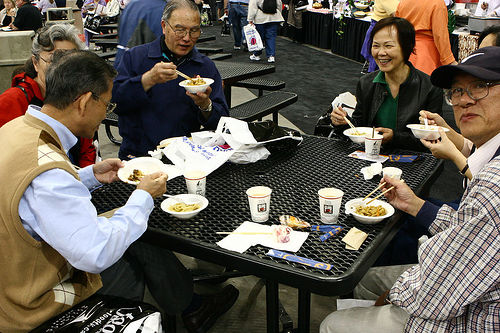
\includegraphics[width=0.4\textwidth]{chapters/ConLL/10459869.jpg}
  \end{center}
  \vspace{1em}
  \begin{subfigure}[t]{0.5\textwidth}
    \textbf{En:} A group of people are eating noodles.\\[0.5ex]
    \textbf{De:} Eine Gruppe von Leuten isst Nudeln.\\[0.5ex]
    \textbf{Fr:} Un groupe de gens mangent des nouilles.\\[0.5ex]
    \textbf{Cs:} Skupina lidí jedí nudle.\\
    \vspace{2em}
    \caption{A translation tuple}
  \end{subfigure}
  \begin{subfigure}[t]{0.5\textwidth}
    \textbf{En:} Several asian people eating around a table.\\[0.5ex]
    \textbf{De:} Drei Männer und zwei Frauen südostasiatischen Aussehens sitzen, aus Schälchen essend, an einem schwarzen, Tisch, auf dem sich u.a. auch Pappbecher und eine Tasche befinden, im Hintergrund sind weitere Personen und Tische.\footnotemark\\
    %\textbf{De:} 3 Männer und 3 Frauen essen zusammen an einem Tisch.
    \caption{A comparable pair}
  \end{subfigure}
  \caption{An example taken from the {\it Translation} and {\it Comparable} portions of the Multi30K dataset. The translation portion (a) contains professional translations of the English captions into German, French, and Czech. The comparable portion (b) consists of five independently crowdsourced English and German descriptions, given only the image. Note that the sentences in (b) convey different information from the English--German translation pair in (a).}\label{fig:data:example}
\end{figure*}


Recently, \cite{gella2017image} proposed to learn both bilingual and multimodal sentence representations using images paired with captions independently collected in English and German. Their results show that bilingual training improves image-sentence ranking performance over a monolingual baseline, and it improves performance on semantic textual similarity benchmarks \cite{agirre2014semeval,agirre2015semeval}. These findings suggest that it may be beneficial to consider another language as another {\it modality} in a monolingual grounded language learning model. In the grounded learning scenario, descriptions of an image in multiple languages can be considered as multiple views of the same or closely related data. These additional views can help overcome the problems of data sparsity, and have practical implications for efficiently collecting image-text datasets in different languages. In real-life applications, many tasks and domains can involve code switching \citep{barman2014code}, which is easier to deal with using a multilingual model. Furthermore, it is more convenient to maintain a single multilingual system than one system for each considered language. However, there is a need for a systematic exploration of the
%the various dimensions of such a system to better understand under
conditions under which it is useful to add additional views of the data. We investigate the impact of the following conditions on the performance of a multilingual grounded language learning model in sentence and image retrieval tasks:
%
\begin{description}
%\setlength\itemsep{0em}
\item[Additional languages.]
Multilingual models have not been explored yet in a multimodal setting. We investigate the contribution of adding more than one language by performing bilingual experiments on English and German (Section~\ref{sec:bi}) as well as adding French and Czech captioned images (Section~\ref{sec:multi}).

\item[Data alignment:] We assess the performance of a multilingual models trained using either captions that are translations of each other, or captions that are independently collected in different languages for the same set of images. The two scenarios are illustrated in Figure~\ref{fig:data:example}. Additionally we consider the setup when non-overlapping sets of images and their captions are collected in different languages. Such disjoint settings have been explored in pivot-based multimodal representation learning \citep{funaki2015image,rajendran2015bridge} or zero-shot multi-modal machine translation \citep{nakayama2017zero}.
We compare translated vs.\ independently collected captions in Sections~\ref{sec:bitrans} and \ref{sec:multitrans}, and overlapping vs.\ disjoint images in Section~\ref{sec:bioverlap}.

\item[High-to-low resource transfer:] In Section~\ref{sec:multitransfer} we investigate whether low-resource languages benefit from jointly training on larger data sets from higher-resource languages. This type of transfer has previously been shown to be effective in machine translation \citep[e.g.,][]{zoph2016transfer}.

\item[Training objective:] In addition to learning to map images to sentences, we study the effect of also learning relationships between captions of the same image in different languages \citep{gella2017image}. We assess the contribution of such a caption--caption ranking objective throughout our experiments.
\end{description}
%
Our results show that multilingual joint training improves upon bilingual joint training, and that grounded sentence representations for a low-resource language can be substantially improved with data from different high-resource languages. Our results suggest that independently-collected captions are more useful than translated captions, for the task of learning multilingual multimodal sentence embeddings. Finally, we recommend to collect captions for the same set of images in multiple languages, due to the benefits of the additional caption--caption ranking objective function.

%Also, through a series of experiments we find that due to the performance benefits of the caption-caption (c2c) objective, it is better to collect captions for the same set of images in multiple languages.
